
\chapter{Current Reversal Theory}
\label{chapter3}



% 3.1.
\section{Perturbation Methods}

% 3.1.1.
\subsection{What is a Perturbation Treatment?}

When it comes to solving differential equations, the ideal scenario 
is that you find an analytic solution, $\psi$. This, however, is generally a 
difficult problem, and especially so in the case of differential equations. A great deal 
of research goes into trying to find analytic solutions to PDEs, 
which is no less true for the Grad-Shafranov equation and its variations. Though 
such efforts are often futile, or require making assumptions about properties of 
your solution which may not be representative of what you're trying to show, 
other means of obtaining the $\Psi(\vec{x})$ for $\vec{x} \in \Omega$ have been developed.

A traditional approach to this is to use some numerical code to approximate solution values. 
There are various codes which exist for this purpose specifically with regards to 
the GSE equation, such as SPEC \cite{spec-code}. These codes come in many flavours - 
some implement a particle simulation, which can provide precision with simulation, 
though are computationally costly. Others exploit various properties of the 
variant of GSE they target and may be computationally more feasible, but are 
restricted in scope, application, and/or reliability because of their assumptions.

A common problem that numerical methods seek to solve is that of time evolution. 
Simulations which evolve a system through time, for obvious reasons, do not discard 
the time dependency component in their derivation of the GSE. 
A common problem that numerical methods are employed to solve is that of time evolution. 
Simulations which evolve a system through time however often require time dependence in the 
system they are trying to solve -- something, if you recall from our derivation of the GSE, is 
not present in our model. This introduces a difficulty for us, as solutions to the GSE explicitly 
represent plasma equilibria, and so we expect no variation of the system with respect to time.

For this thesis, given the availability of an analytic solution to a variation of 
the GSE that specifically relates to current reversals, we employ a hybrid approach. 
In our simulation we wish to observe changes in the system through a current ramp down
- this necessitates a time dependency component to our solution. However, there are 
a couple points to note:
\begin{itemize}
    \item Time evolution simulations are expensive
    \item Existing literature on time evolution GSE do not take into account the possibility for current 
    reversal
    \item The GSH variant we utilise (which has yet to be introduced) is not time dependent, i.e., 
    was not derived taking into account a time component
\end{itemize}

There are a couple possible avenues we could explore from here. We could implement a numerical code 
for the time evolution, for example a particle simulation, however this is for all intents and purposes
computationally infeasible given the hardware available (a beloved but dilapidated Thinkpad T440p). We could 
attempt to find an analytic solution to the GSE with time dependence (or an approximation to one),
but given the mountain of research existing in this space and the relative inexperience 
of the author, this would likely be a futile task. The third, and most lucrative option, 
is to use an existing analytic solution to a variation of the GSE that accounts for 
current reversal, and explore if small changes to its state
are sufficiently ``good enough'' approximations of our system that it can be used to make 
statements about experimental data.

This is where perturbation theory comes in. Intuitively we would expect a 
plasma to vary ``smoothly'' - nature rarely behaves in instantaneous ways. The 
analytic solution we will soon have describes the instantaneous state (a slice in time) of 
our plasma's state. We may anticipate then that if we were to change something 
in our system by a ``sufficiently small amount'' (we will later comment on what exactly is meant by sufficiently small), 
that our system may react to that change of state in a way that approximates how it would if it 
were really varying through time. 

\subsubsection{Resistivity Note}
When we derived the ideal MHD equations we compared them to the resistive MHD model, noting that 
the removal of resistivity would be an important simplification to note. Here we see its importance, as 
we are now allowing our system to vary with respect to time, which means that there exists some time scale 
for which resistive effects will begin to impact the behaviour of our plasma. 

Our model assumes the ideal MHD assumptions however, which includes dropping resistivity, and so the effect 
of these resistive instabilities is lost in our model. The question of whether these effects are significant 
enough to affect the accuracy of our time evolution is one we hope to answer when we come to reviewing our simulations in 
chapter \ref{chapter5}.

A perhaps more intuitive analogy is that of swimming. Imagine you are stationary sitting 
at the bottom of a pool, and you are looking at your arm extended out in front of you. 
Focus on the feeling of the water moving around your arm - this will emulate the resistivity 
that electrons would feel. If you move your arm abruptly, 
perhaps in a cutting motion, then you will feel the pressure of the water push against 
your arm, and that might affect how quickly you can move your arm, or if the current of the water is 
particularly strong, perhaps you notice your arm move not in the direction you intended. Perhaps 
you also have to use more energy to move your arm than you intended, so it doesn't go as far. 
Now imagine instead that you don't abruptly cut, but instead, very slowly, almost 
imperceptibly, move your arm through the water. In this case you may not be aware of any resistance at all 
- there is no sensation of resistance, your arm moves exactly as fast as you expect it to, and you use exactly 
the amount of energy to move it as you expected. However, if you do this for long enough, perhaps you 
will begin to notice the effects more and more. Or maybe by now you'll realise you're out of breath and need 
to resurface. An instructive graphic is below.

\begin{figure}[h!]
    \centering
    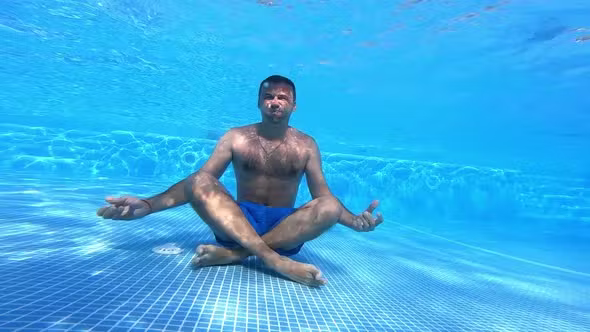
\includegraphics[scale=0.6]{imgs/c3/pool.png}
    \caption{Demonstrative graphic for conducting a resistivity experiment at the bottom of a pool.}
\end{figure}
\newpage

We will have the ability to determine the 
state of our system for some given parameters, and so the question becomes: can 
we vary our input in a way such that the behaviour of the analytic solution to 
the GSH is an approximation of a time evolution of the plasma. We are able to compare 
our results to experimental data, and then exploit our work to answer further questions.



% 3.1.2.
\subsection{Regular Perturbation Theory}

At the heart of perturbation theory is the manipulation of functions by some small amount to achieve a goal. A familiar 
perturbation is the taylor expansion - if we have some function $f(x)$, then we can use $n^{\text{th}}$ order derivatives to approximate 
the value of the function for some perturbation $a$
\begin{equation*}
    f(x) = \sum_{n = 0}^{\infty} \frac{f^{(n)}(a)}{n!} (x - a)^n
\end{equation*}
In a similar spirit, we can expand a function $f(x)$ around a point $x = a$ by some $\epsilon$ amount
$$f(a + \epsilon) = f(a) + \epsilon \dv{f}{x}(a) + \frac{1}{2} \epsilon^2 \dv[2]{f}{x}(a) + \dots$$
and it is this sentiment that is what drives perturbation theory - that some small change in input of a function can result 
in small changes in the output of that function. This is obviously not the case for all functions - immediately we see that this 
fails for anything that is not differentiable, an in general if we wish to make an approximation to the $n^{\text{th}}$ degree then 
we need our function to at least be $f \in C^n$ \cite{perturbation-basics}. 

When it comes to PDEs, regular perturbation theory can be used to find solutions to unknown functions. The general process is \cite{perturbation-basics}:
\begin{enumerate}
    \item Set $\epsilon = 0$, solve the resulting system (i.e., a solution for $f_0$ effectively)
    \item Perturb the system by $\epsilon$ (i.e., go back and expand the system in terms of some $\epsilon > 0$)
    \item Let the (unknown) solution to the new perturbed system be given as
    $$f_0 + \epsilon f_1 + \epsilon^2 f_2 + \dots$$
    \item Expand the PDE in terms of $\epsilon$. Collect like powers of $\epsilon$ and solve these are their own systems
    \item Collate solutions for each $f_i$ as found for their respective powers of $\epsilon$ - this is your approximation 
    to the analytic solution to the PDE
\end{enumerate}

\noindent
Formally then we can state that, given a differential equation
$$F(D^{k} u(x), D^{k-1}u(x), \dots, Du(x), x) = 0$$
that an expansion for $u$ can be given
$$u(x) = u_0(x) + \epsilon u_1(x) + \epsilon^2 u_2(x) + \dots$$
If we were able to reason about all the derivatives of $u$ (and they exist), then in the ideal case we 
can retrieve an analytic solution to the PDE. However, if instead the function is not $C^{\infty}$, or perhaps 
becomes too difficult to analytically solve, we could instead solve for an approximate solution by instead expanding, for 
example, to the second order:
$$u(x) = u_0(x) + \epsilon u_1(x) + \epsilon^2 u_2(x) + \mathcal{O}(\epsilon^2)$$

\subsubsection{Example}
Here we will follow an example provided by \cite{perturbation-example}, which emphasis the utility of perturbation methods in solving 
differential equations. 

Let a body have mass $m$ with initial velocity $v_0$. It moves in a straight line, however there is a resistive force opposing its motion 
with magnitude $av - bv^2$, where $v(\tau)$ describes the velocity of the object. We assume $b \ll a$ are constants, and Newton's law provides
$$m \dv{v}{\tau} = -av + bv^2$$
with the boundary condition
$$v(0) = v_0$$
We can make this system dimensionless by making a change of variables with $y = v / v_0$ and $t = \tau / (m / a)$, giving us the new system
$$\dv{y}{t} = -y + \epsilon y^2$$
with boundary condition
$$y(0) = 1$$
where $\epsilon \equiv (b v_0) / a \ll 1$. Now with our dimensionless model we can begin our perturbations. 
Instead of opting for an analytic solution, 
we'll use an approximation, so we will expand as such:
$$y(t) = y_0(t) + \epsilon y_1(t) + \epsilon^2 y_2(t)$$
and ignore any $\mathcal{O}(\epsilon^3)$ terms. Substituting this into our dimensionless model gives
\begin{align*}
    \dv{y}{t} &= -y + \epsilon y^2 \\
    y_0' + \epsilon y_1' + \epsilon^2 y_2' &= -(y_0 + \epsilon y_1 + \epsilon^2 y_2) + \epsilon \left (y_0 + \epsilon y_1 + \epsilon^2 y_2 \right )^2
\end{align*}
Then, we next collect similar powers of $\epsilon$ (representing different orders of approximation), which we observe is a series of 
linear ODEs:
\begin{align*}
    y_0' &= -y_0 \\
    y_1' &= -y_1 + y_0^2 \\
    y_2' &= -y_2 + 2y_0 y_1
\end{align*}
The initial condition also tells us that $y_0 (0) + \epsilon y_1(0) + \epsilon^2 y_2(0) = 1$, but, as we know $y_0(0) = 1$, 
we also get that $y_1(0) = y_2(0) = 0$. Thus, we have a series of ODEs with initial conditions specified for each, which 
harks back to first year calculus courses. We readily have solutions available for each of the ODEs:
\begin{align*}
    y_0(t) &= e^{-t} \\
    y_1(t) &= e^{-t} - e^{-2t} \\
    y_2(t) &= e^{-t} - e^{-2t} + e^{-3t}
\end{align*}
and thus, our approximate solution to $y$ can be given
$$y(t) \approx e^{-t} + \epsilon(e^{-t} - e^{-2t}) + \epsilon^2 (e^{-t} - e^{-2t} + e^{-3t})$$
As a form of validation, with omnipotent knowledge we can state that the actual solution to the original equation can 
be given as 
$$y(t) = \frac{e^{-t}}{1 + \epsilon(e^{-t} - 1)}$$
which has the Taylor series expansion (in $\epsilon$):
$$y(t) = e^{-t} + \epsilon(e^{-t} - e^{-2t}) + \epsilon^2(e^{-t} - e^{-2t} + e^{-3t}) + \mathcal{O}(\epsilon^3)$$
which is exactly what our perturbation approximation determined \cite{perturbation-example}. A cool demonstration, if we can say so ourselves!

While we won't be performing such an in depth perturbation treatment of the MHD equations themselves, it is this spirit 
of approximation via perturbation which we will carry through our work, and keep in mind when it comes to our simulations.

% 3.1.3.
\subsection{Ideal MHD Perturbation}

At the beginning of this thesis we introduced it as being interdisciplenary in nature. 
Keeping in that spirit, at times here we will put on our physicists cap and 
seemingly arbitrarily remove terms we no longer wish to have. We 
kindly ask that any mathematicians reading these sections avert their gaze in such 
times so as to maintain sanity.

In Chapter \ref{chapter2} we derived the ideal MHD equations, and their subsequent reduction, used in GSE, given:
\begin{align}
    \vec{j} \times \vec{B} &= \nabla p \\
    \mu_0 \vec{j} &= \nabla \times \vec{B} \\
    \nabla \cdot \vec{B} &= 0
\end{align}
These by note are time independent. We wish to look at the 
effect of some small ($\epsilon > 0$) time perturbation to the original system however, and so 
will return to their derivation, this time without discarding the time component. Consider the pre-GSE ideal MHD equations again, 
as given in (\eqref{ideal-mhd-first} - \eqref{ideal-mhd-last})
\begin{align*}
    \frac{\DD}{\DD t} \rho &= -\rho \nabla \cdot \vec{u} \\
    \rho \frac{\DD}{\DD t} \vec{u} &= -\nabla p + \vec{j} \times \vec{B}\\
    \frac{\DD}{\DD t} p  &= -\gamma p \nabla \cdot \vec{u} \\
    \shortintertext{with the assumptions}
    \pdv{\vec{B}}{t} &= -\nabla \times \vec{E} \\
    \mu_0 \vec{j} &= \nabla \times \vec{B} \\
    \vec{E} + \vec{u} \times \vec{B} &= 0 
\end{align*}

We will apply our perturbation treatment to the first three equations of these (the continuity equation, momentum equation, and 
energy equation), using the assumptions to aid us. We will being with the continuity equation.

\subsubsection{Continuity Equation Time Perturbation}
We restate the continuity equation:
\begin{equation*}
    \frac{\DD}{\DD t} \rho = -\rho \nabla \cdot \vec{u}
\end{equation*}
Here we have two functions, $\rho$ and $\vec{u}$, which are both functions of three dimension in space and one of time, i.e.
\begin{align*}
    \rho &:= \rho(\vec{r}, t) \\
    \vec{u} &:= \vec{u}(\vec{r}, t)
\end{align*}
where $\vec{r} \in \R^3, t \in \R$. Here (and throughout these perturbation treatments) we will decouple the time dependency by 
assuming it to be some epsilon perturbation from an initial state. For example, for mass density ($\rho$), we can let $\rho_0$ 
describe some initial state that is only dependent on space, and $\rho_1$ a perturbation component similarly dependent only on space. Let $\epsilon_{\rho} < 0$ be some small perturbation factor
for mass density, and $t$ be the time evolved. Then we prescribe a time-linear perturbation expansion as such:
\begin{align*}
    \rho(\vec{r}, t) &= \rho_0(\vec{r}) + \epsilon_\rho t \rho_1(\vec{r}) + \mathcal{O}(\epsilon_\rho^2)
    \shortintertext{and analogously:}
    \vec{u}(\vec{r}, t) &= \vec{u}_0(\vec{r}) + \epsilon_u t \vec{u}_1 (\vec{r}) + \mathcal{O}(\epsilon_u^2)
\end{align*}
Here the $t$ term effectively acts as a scaling factor on top of $\epsilon$. We have also dropped any $\epsilon$ terms of order 
greater than $1$ in our approximation, that is to say, if we were to be accurate our expansion would actually be:
\begin{align*}
    \rho(\vec{r}, t) &= \rho_0(\vec{r}) + \epsilon_\rho t \rho_1(\vec{r}) + \epsilon^2_\rho t \rho_2(\vec{r}) + \dots \\
    \vec{u}(\vec{r}, t) &= \vec{u}_0(\vec{r}) + \epsilon_u t \vec{u}_1 (\vec{r}) + \epsilon^2_{u} t \vec{u}_2(\vec{r}) + \dots
\end{align*}
As we said at the start of this chapter however, this is an interdisciplenary thesis, and the above is an example of us putting on our 
physicist cap and deciding to remove ``unnecessary'' complexity. Physically we can justify this dropping of terms as we would expect terms of 
greater order to contribute diminishingly to our system. That is to say, on the time scales we are considering, an approximation of up to $\epsilon$ 
should be sufficient for experimental comparisons. As such, we need only to reason about that, and drop any terms on order of $\mathcal{O}(\epsilon^2)$.
We substitute these perturbation expansions into our equation. For brevity we will drop function parameters in our notation, and 
first begin with an expansion of the $\rho$ term:
\begin{align*}
    \shortintertext{\textit{LHS:}}
    \frac{\DD}{\DD t} \rho &= \left ( \pdv{t} + \vec{u} \cdot \nabla \right ) \rho \\
    &= \pdv{t} \rho + \vec{u} \cdot (\nabla \rho) \\
    &= \pdv{t} (\rho_0 + \epsilon_\rho t \rho_1) + \vec{u} \cdot (\nabla (\rho_0 + \epsilon_\rho t \rho_1)) \\
    &= \pdv{t}\rho_0 + \epsilon_\rho \rho_1 + \vec{u} \cdot (\nabla \rho_0) + \epsilon_\rho t \vec{u} \cdot (\nabla \rho_1) \\
    \shortintertext{noting that $\rho_0$ is not a function of time}
    &= \epsilon_\rho \rho_1 + \vec{u} \cdot (\nabla \rho_0) + \epsilon_\rho t \vec{u} \cdot (\nabla \rho_1)
    \shortintertext{\textit{RHS:}}
    -\rho \nabla \cdot \vec{u} &= -(\rho_0 + \epsilon_\rho t \rho_1) (\nabla \cdot \vec{u}) \\
    &= -\rho_0 (\nabla \cdot \vec{u}) - \epsilon_\rho t \rho_1 (\nabla \cdot \vec{u})
\end{align*}
\begin{align*}
    \shortintertext{\textit{Combined:}}
    \frac{\DD}{\DD t} \rho &= -\rho \nabla \cdot \vec{u} \\
    \epsilon_\rho \rho_1 + \vec{u} \cdot (\nabla \rho_0) + \epsilon_\rho t \vec{u} \cdot (\nabla \rho_1) &= -\rho_0 (\nabla \cdot \vec{u}) - \epsilon_\rho t \rho_1 (\nabla \cdot \vec{u}) \\
    \epsilon_\rho \rho_1 + \epsilon_\rho t \left [ \vec{u} \cdot (\nabla \rho_1) + \rho_1 (\nabla \cdot \vec{u}) \right ] &+ [\rho_0 (\nabla \cdot \vec{u}) + \vec{u} \cdot (\nabla \rho_0)] = 0 \\
    \epsilon_\rho \rho_1 + \nabla \cdot (\rho_0 \vec{u}) + \epsilon_\rho t [\nabla \cdot (\rho_1 \vec{u})] &= 0
\end{align*}
Here we have used the divergence property $\nabla \cdot (f\vec{v}) = (\nabla f) \cdot \vec{v} + f(\nabla \cdot \vec{v})$. Note that for the 
Grad-Shafranov equation we usually (and we shall) assume an incompressible fluid, which mathematically is significant as it gives us the property 
that $\nabla \cdot (\rho \vec{u}) = 0$. From the above we immediately get that $\epsilon_\rho \rho_1 = 0$, which just tells us that the time component 
we introduced has no effect on the system, given the assumptions we make. This is excellent news for us, as it means that small perturbations 
in our system in a manner that emulates a time evolution should not affect the accuracy of our model, at least insofar as the effects of the 
continuity equation are concerned, and up to a term of $\mathcal{O}(\epsilon^2)$. To be confident that we can do this for the Grad-Shafranov equation on a whole, we need to repeat this process for 
the other ideal MHD equations. Next we'll look at the momentum equation.

\subsubsection{Momentum Equation}
We restate the momentum equation here:
\begin{equation*}
    \rho \frac{\DD}{\DD t}\vec{u} = -\nabla \rho + \vec{j} \times \vec{B}
\end{equation*}
We will follow the same process as we did for the continuity equation. Here we have four equations, however, by introducing one of 
our GSE assumptions we can reduce this to three immediately. For GSE we assume that our fluid has no velocity, i.e. $\vec{u} = 0$, which 
gives us that $\frac{\DD}{\DD t} \vec{u} = 0$. Thus the equation we actually have to expand is:
\begin{equation*}
    0 = -\nabla \rho + \vec{j} \times \vec{B}
\end{equation*}
The three equations we have are each functions of $\vec{r} \in \R^3$ and $t \in \R$, and can be linearly perturbed in time as we did earlier. As such:
\begin{align*}
    \rho(\vec{r}, t) &:= \rho_0(\vec{r}) + \epsilon_\rho t \rho_1(\vec{r}) + \mathcal{O}(\epsilon_\rho^2) \\
    \vec{B}(\vec{r}, t) &:= \vec{B}_0(\vec{r}) + \epsilon_B t \vec{B}_1(\vec{r}) + \mathcal{O}(\epsilon_B^2) \\
    \vec{j}(\vec{r}, t) &:= \vec{j}_0(\vec{r}) + \epsilon_j t \vec{j}_1(\vec{r}) + \mathcal{O}(\epsilon_j^2)
\end{align*}
Making these substitutions into the momentum equation:
\begin{align*}
    \nabla \rho &= \vec{j} \times \vec{B} \\
    \nabla (\rho_0 + \epsilon_\rho t \rho_1) &= \vec{j} \times (\vec{B}_0 + \epsilon_B t \vec{B}_1) \\
    (\nabla \rho_0) + \epsilon_\rho t (\nabla \rho_1) &= (\vec{j} \times \vec{B}_0) + \epsilon_B t (\vec{j} \times \vec{B}_1) \\
    (\nabla \rho_0) + \epsilon_\rho t (\nabla \rho_1) = [(\vec{j}_0 \times \vec{B}_0) + \epsilon_j t (\vec{j}_1 &\times \vec{B}_0)] + \epsilon_B t [(\vec{j}_0 \times \vec{B}_1) + \epsilon_j t (\vec{j}_1 \times \vec{B}_1)] \\
    (\nabla \rho_0) + \epsilon_\rho t (\nabla \rho_1) &= \vec{j}_0 \times \vec{B}_0 + \epsilon_j \epsilon_B t^2 (\vec{j}_1 \times \vec{B}_1)
\end{align*}
If we collate terms of like order, we get 
\begin{align*}
    \nabla \rho_0 &= \vec{j}_0 \times \vec{B}_0 \\
    \nabla \rho_1 &= \frac{\epsilon_j \epsilon_B}{\epsilon_\rho} t (\vec{j}_1 \times \vec{B}_1) 
\end{align*}
both of which look remarkably like the original momentum equation; an observation which is not to be mistaken for coincidence. Notably, when we take our 
evolution over ``small enough'' time scales, the perturbation components here disappear entirely, and we are left with the version of the 
momentum equation which is used in the regular equilibrium-state derivation of the Grad-Shafranov equation. As such, we would anticipate that 
small time perturbations associated with the effects of the momentum equation will introduce ``small'' errors in the resulting GSE solution, though 
(and as we hope to observe through experiment), hopefully imperceptibly so - as the above expansion seems to suggest.  

\subsubsection{The Other Ideal MHD Equations}
Isaac Newton is quoted as saying ``it causeth my head to ache'', which he is claimed to have said in reference to perturbation expansions 
in trying to determine the orbit of the Moon \cite{newton-headache}. Hopefully understandably, we ask that the reader excuse our omitting the working for the more involved of the ideal MHD equations, 
as to write it all down here would be to commit an expositionary crime. The expansion of the remaining equations however leads to a similar outcome 
as we found with the continuity equation and the momentum equation - that, up to an $\epsilon$ factor, the ideal MHD equations do not show significant deviation 
from their equilibrium counterparts. 

\subsubsection{Significance}
The purpose of this exercise was to provide some theoretical justification for the simulations we will later run. By showing that we can 
approximate a linear time evolution of the ideal MHD equations using states of equilibrium, we have shown that the GSE will be resistant 
to such a treatment itself. What we have not done is show that GSE itself can be evolved through time in an accurate manner. We are, knowingly, 
introducing errors into our system -- but the hope is that the errors introduced will be insignificant with respect to the measurements we seek to make. 
This is the nature of mathematical modelling.

It is important to remark that the GSE is an equilibrium model - it is constructed under the assumptions of plasma equilibrium, and as we've 
already remarked on for resistivity, essentially ``wishes away'' many of the physical effects that would otherwise be introduced by some plasma which actually does 
change with respect to time. To that extent, 
it could be considered tomfoolery (which, for what it's worth, does befit the author) to assume that the work we've done is a guarantee that 
we can simply take equilibrium solutions to the GSE and assume that one is an evolution of the other in time, while still maintaining physicality.

While this may seem rather bleak / unpromising (after all, we are conceding that the model we have is not an entirely accurate 
physical representation of what's going on), the question we concern ourselves with is whether it is good enough to explain 
the observed runaway electron phenomena. To that extent, we will next introduce a variation of the Grad-Shafranov equation, 
solutions for which describe current reversal equilibrium configurations (CREC). We posit then that, if we take a 
solution to this system and perturb the current density profile by some small $\epsilon$ in time, then the resulting 
change in the GSH solution will be a sufficiently accurate representation of a physical system so as to explain the 
presence of excess runaway electrons.

% 3.2.
\section{Grad-Shafranov-Helmholtz Equation}

The Grad-Shafranov equation, in its default state (as we have derived it), does not account for the possibility of current 
reversal equilibrium configurations (CRECs). That is to say, it does not permit anti-parallel current channels in an equilibrium state. 
This is problematic, as this is one of the behaviours we are seeking to identify in simulation. In the last 20 years work has been done on 
modelling such configurations, and analytic results have become more abundant \cite{wang-analytic-solution}, \cite{crec-work-1}, \cite{crec-work-2}.
For our purposes, we are interested in work done by Wang and Yu in deriving an analytic solution to a variant of the Grad-Shafranov equation 
known as the Grad-Shafranov-Helmholtz equation, which is capable of supporting CRECs. In this section we'll present their work, provide a 
brief derivation, and highlight the components that will be important for our simulations (the current density and pressure density profiles). 
Then we'll demonstrate an ability to recreate Wang's results.

% 3.2.1.
\subsection{Equation and Derivation}

The work here will largely follow the paper by Wang and Yu \cite{wang-analytic-solution},
with some key notes and modifications. We are by now familiar with the GSE:
\begin{equation}
    x \pdv{x} \left ( \frac{1}{x} \pdv{\Psi}{x} \right ) + \pdv[2]{\Psi}{z} = -\mu_0 x^2 \pdv{p}{\Psi} - \mu_0^2 f(\Psi) \pdv{f}{\Psi}
\end{equation}

Wang provides a slightly different (though equivalent) formulation:
\begin{proposition}
    Let $R_0$ and $a$ describe the major and minor radius. $B_0$ is then the magnetic axis, which Wang takes to be 
    the strength of the magnetic field at $R = R_0$. Additionally, we let $\psi = \Psi / (B_0 a^2)$ be the 
    normalised poloidal magnetic flux, and we let $x = R/a$ and $z = Z/a$. For flux fucntions, we let $\beta(\psi) = (2 \mu_0 p(\psi))/B_0^2$, 
    $g(\psi) = F(\psi) / (B_0 a)$ and $j_\phi = (J_{\phi} \mu_0 a) / B_0$, where $J_{\phi}$ is the toroidal current density. 
    The GSE can then equivalently be stated:
    \begin{align}
        \label{wang-gse} \left ( x \pdv{x} \frac{1}{x} \pdv{x} + \pdv[2]{z} \right ) \psi &= -\frac{1}{2} x^2 \dv{\beta}{\psi} - \frac{1}{2}\dv{g^2}{\psi} = -x j_{\phi} \\
        \intertext{where}
        \label{a1} a_1 &= -\frac{1}{2} \dv{\beta}{\psi} \\
        \label{a2-alpha} -a_2 - \alpha^2 \psi &= -\frac{1}{2} \dv{g^2}{\psi}
    \end{align}
    Additionally we impose the boundary condition $\psi |_b = 0$. 
\end{proposition} 

\begin{remark}
    We highlight here the parameter tuple $(a_1, a_2, \alpha)$. We will see soon that 
    these parameters can be used to determine our system. For now we simply note their 
    significance so that the reader (that's you!) may pay them special attention through the rest of the following working.
\end{remark}

\begin{definition}[Helmholtz Equation]
    A Helmholtz equation is a problem associated with the below form
    $$\nabla^2 f = -k^2 f$$
    where $\nabla^2$ is the Laplace operator, $k^2$ is the eigenvalue, and $f$ is an eigenfunction.
\end{definition}
The equation we have in \ref{wang-gse} is in fact just the Grad-Shafranov equation. If, instead of a flux function $\psi$, we consider 
a toroidal vector potential factor $A = \psi / x$, then the GSE formulation given above reduces to a separate system, which can be identified 
as being Helmholtz:
\begin{align}
    \label{wang-gsh} \left ( \frac{1}{x} \pdv{x} x \pdv{x} + \pdv[2]{z} - \frac{1}{x^2} \right ) A + \alpha^2 A &= a_1 x - a_2 \frac{1}{x} \\
    A |_b &= 0
\end{align}

We then seek a solution $\psi(x,z)$ for equation \ref{wang-gse}, which satisfies the above conditions in \ref{wang-gsh}. Wang provides one:
\begin{proposition}
    The below is a solution to the GSH as given above
    \begin{equation}
        \label{gsh-solution} \psi(x,z) = x \sum_{n = 1}^{\infty} \sum_{l = 0}^{\infty} \frac{(-1)^l 2 a_n^u}{kv_la_n^d (\alpha^2 - \lambda_{n,l}^2)} \left [ c_n J_1(\mu_n x) + N_1(\mu_n x)\right ] \cos(v_l z)
    \end{equation}
    where here $J_\alpha$ are Bessel functions of the first kind, and $N_\alpha$ are Bessel functions of the second kind. Some of these other terms we will for now 
    leave unexplained, as we will cover them in the derivation. 
\end{proposition}

\subsubsection{Derivation}
We will assume a cylindrical coordinate system, and consider our boundary conditions to be a rectangular cross section. We will 
take $x \in [x_0 - a, x_0 + a]$ and $z \in [-k, k]$, where $k$ is an elongation constant which determines the ellipticity of the cross section. 
With this in mind, the equivalent problem to \ref{wang-gsh} is the system
\begin{align}
    \label{4a} \left ( \frac{1}{x} \pdv{x} x \pdv{x} + \pdv[2]{z} - \frac{1}{x^2} \right ) U + \lambda^2 U &= 0 \\
    \label{4b} U(x_0 - a, z) = U(x_0 + a, z) &= 0 \\
    \label{4c} U(x, -k) = U(x, k) &= 0
\end{align}
If we begin by assuming that a solution is of the form $U(x,z) = \mathcal{R}(x) \mathcal{Z}(z)$, then we can describe it as an 
orthogonal system of eigenfunctions, and make a Fourier expansion as such:
\begin{align}
    \label{10a} A(x,z) &= \sum_{n = 1}^{\infty} \sum_{l = 0}^{\infty} A_{n,l} \mathcal{R}_n(x) \mathcal{Z}_l(z) \\
    \label{10b} a_1 x - a_2 \frac{1}{x} &= \sum_{n = 1}^{\infty} \sum_{l = 0}^{\infty} f_{n,l} \mathcal{R}_n(x) \mathcal{Z}_l(z)
\end{align}
Equations \ref{10a} and \ref{10b} can be substituted into \ref{wang-gsh}, Wang found an explicit form for $A_{n,l}$:
\begin{equation}
    \label{a-form} A_{n,l} = \frac{f_{n,l}}{\alpha^2 - \lambda_{n,l}^2} = \frac{(-1)^l 2a_n^u}{kv_l a_n^d (\alpha^2 - \lambda_{n,l}^2)}
\end{equation}
Thus, we need to reason about the values $\mathcal{R}_n(x)$ and  $\mathcal{Z}_l(z)$. 
If we introduce constants $v^2$ and $\mu^2$ such that $\lambda^2 = v^2 + \mu^2$ (a result of $\mathcal{Z}$ and $\mathcal{R}$ being orthogonal), Wang found the relations
\begin{align}
    \label{5a} \dv[2]{\mathcal{Z}}{x} + v^2 \mathcal{Z} &= 0 \\
    \label{5b} \mathcal{Z}(-k) = \mathcal{Z}(k) &= 0 \\
    \label{5c} \dv[2]{\mathcal{R}}{x} + \frac{1}{2} \dv{\mathcal{R}}{x} + \left ( \mu^2 - \frac{1}{x^2} \right ) \mathcal{R} &= 0 \\
    \label{5d} \mathcal{R}(x_0 - a) = \mathcal{R}(x_0 + 1) &= 0
\end{align}
Equations \ref{5a} and \ref{5b} are an eigenvalue problem, and provide the following eigenvalues and eigenfunctions
\begin{align}
    v_l &= \frac{1}{k} (l + \frac{1}{2}) \pi \\
    \label{z-func} \mathcal{Z}_l(z) &= \cos(v_l z)
\end{align}
with $l \in \Z_{\ge 0}$. Similarly, equation \ref{5c} with \ref{5d} represent another eigenvalue problem. The eigenfunctions 
are given as
\begin{equation}
    \label{r-func} \mathcal{R}_n(x) = c_n J_1(\mu_n x) + N_1(\mu_n x)
\end{equation}
where $n \in \Z_{\ge 1}$. Here, however, we don't have an explicit form for the eigenvalues $\mu_n$. Instead, 
$\mu_n$ is described as being the zeros of the function
\begin{equation}
    -J_1(\mu_n (x_0 + a)) \frac{N_1(\mu_n (x_0 - a))}{J_1 (\mu_n (x_0 - a))} + N_1(\mu_n (x_0 + 1)) = 0
\end{equation}
where
$$c_n = -\frac{N_1(\mu_n (x_0 - a))}{J_1 (\mu_n (x_0 - a))}$$
Thus we can summarise the eigenvalues and eigenfunctions of \ref{4a} - \ref{4c} are given by
\begin{align}
    \lambda_{n,l}^2 &= v_l^2 + \mu_n^2 \\
    U_{n,l}(x,z) &= \mathcal{R}_n(x) \mathcal{Z}_l(z)
\end{align}
Thus we have an explicit form for the eigenfunctions we required in \ref{a-form}. We can also now 
provide expressions for the until now unknown variables in \ref{a-form}, the derivations for which are 
given by Wang in an earlier paper \cite{wang-precursor}. We provide them en masse here:
\begin{align}
    e_n^u(x) &= \frac{1}{\mu_n} \left [ a_1 x^2 (c_n J_2(\mu_n x) + N_2(\mu_n x)) + a_2 (c_n J_0 (\mu_n x) + N_0(\mu_n x)) \right ] \\
    a_n^u &= [e_n^u(x)]_{x_0 - a}^{x_0 + a} \\
    e_n^d(x) &= -\frac{1}{2} x^2 N_0(\mu_n x) N_2(\mu_n x) - \frac{1}{2} c_n^2 x^2 J_0(\mu_n x) J_2(\mu_n x) \\
    \notag &+ c_n \left [ \frac{1}{2}x^2 (J_0(\mu_n x) - J_2(\mu_n x) )N_0(\mu_n x) - \frac{1}{\mu_n} x J_0(\mu_n x) N_1(\mu_n x) \right ] \\
    a_n^d &= [a_n^d (x)]_{x_0-a}^{x_0+a}
\end{align}
Note here that the superscripts $u$ and $d$ are not indices, but are just used to distinguish between variables. Thus, to show that $\psi(x,z)$ as
provided in \ref{gsh-solution} is a solution, we simply substitute equations \ref{z-func}, \ref{r-func} and \ref{a-form} into \ref{10b}.

% 3.2.3.
\subsection{Current Density and Pressure Density}
We have an explicit formula for the poloidal magnetic flux function $\psi$ (albeit normalised for our case), but we remain to have an 
expression for our current density and pressure density profiles.

\subsubsection{Pressure Density Profile}
In a small note below equation (16c) of \cite{wang-analytic-solution}, an expression for the plasma pressure is given as
\begin{equation}
    \label{pressure-profile} \beta(x,z) = \beta_0 - 2a_1 \psi(x,z)
\end{equation}
where $\beta_0$ is chosen such that the minimum of the expression is zero for the domain (this just ensures that it's not possible 
to have negative pressures).

\subsubsection{Current Density Profile}
Equation \ref{wang-gse} relates the toroidal current density to our parameters $a_1, a_2$ and $\alpha$. As we know 
all other components here, we can draw the toroidal current density from this. In doing so, recall notably equations \ref{a1} and \ref{a2-alpha}.
\begin{align}
    \notag -xj_{\phi}(x,z) &= -\frac{1}{2}x^2 \dv{\beta}{\psi} - \frac{1}{2} \dv{g^2}{\psi} \\
    \notag -xj_{\phi}(x,z) &= a_1 x^2 - a_2 - \alpha^2 \psi(x,z) \\
    \label{current-profile} \implies j_{\phi}(x,z) &= -a_1 x + \frac{1}{x} a_2 + \frac{\alpha^2}{x} \psi(x,z)
\end{align}

\begin{remark}
    As we stated toward the start of this chapter, three parameters appear crucial to this system - $(a_1, a_2, \alpha)$. We see that, in fact, 
    the entirety of our system can be determined by them, as any other variables are configuration variables for the tokamak. Thus, if we 
    the values $(a_1, a_2, \alpha)$ can be used to calculate the poloidal magnetic flux, the current density profile, and the 
    pressure density profile.
\end{remark}

% 3.3.
\section{Simulations}
At this point, we are able to describe the poloidal magnetic field flux function, current density profile, and pressure density profile for a 
tokamak under the restrictions of the GSH model. However, we are only able to do this if we are given some set of parameter, $(a_1, a_2, \alpha)$. 
In the next chapter we will deal with the question of deriving these parameters for a given current density profile, but for now we can simply reproduce 
the results given by Wang in section 3 of \cite{wang-analytic-solution}.

\begin{figure}[h!]
    \centering
    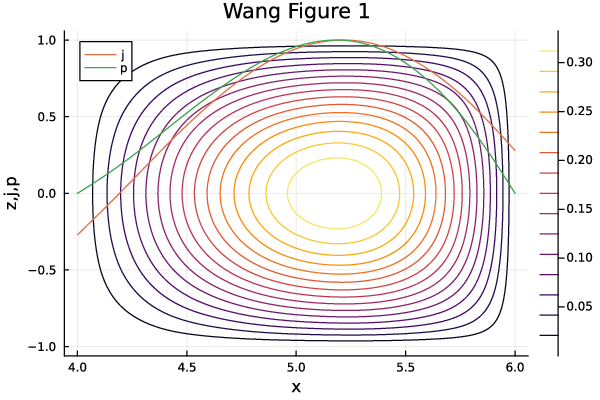
\includegraphics[scale=0.7]{imgs/c3/wang-fig-1.png}
    \caption{Figure 1 of \cite{wang-analytic-solution}. Here, there parameters are $(a_1, a_2, \alpha) = (-0.04531, -1.0808, 2.1683)$, 
    where the minor radius $a = 1$, the elongation is $k = 1$, and the major radius is taken to be $R = 5$.}
\end{figure}
